%!TEX program = xelatex

\documentclass[a4paper, openany, oneside]{memoir}
\usepackage[no-math]{fontspec}
\usepackage{pgfplots}
\pgfplotsset{compat=newest}
\usepackage{commath}
\usepackage{mathtools}
\usepackage{amssymb}
\usepackage{amsthm}
\usepackage{booktabs}
\usepackage{mathtools}
\usepackage{xcolor}
\usepackage[separate-uncertainty=true, per-mode=symbol]{siunitx}
\usepackage[noabbrev, capitalize]{cleveref}
\usepackage{listings}
\usepackage[american inductor, european resistor]{circuitikz}
\usepackage{amsmath}
\usepackage{amsfonts}
\usepackage{ifxetex}
\usepackage[dutch,english]{babel}
\usepackage[backend=bibtexu,texencoding=utf8,bibencoding=utf8,style=ieee,sortlocale=en_GB,language=auto]{biblatex}
\usepackage[strict,autostyle]{csquotes}
\usepackage{parskip}
\usepackage{import}
\usepackage{standalone}
\usepackage{hyperref}
%\usepackage[toc,title,titletoc]{appendix}

\ifxetex{} % Fonts laden in het geval dat je met Xetex compiled
    \usepackage{fontspec}
    \defaultfontfeatures{Ligatures=TeX} % To support LaTeX quoting style
    \setromanfont{Palatino Linotype} % Tover ergens in Font mapje in root.
    \setmonofont{Source Code Pro}
\else % Terug val in standaard pdflatex tool chain. Geen ondersteuning voor OTT fonts
    \usepackage[T1]{fontenc}
    \usepackage[utf8]{inputenc}
\fi
\newcommand{\references}[1]{\begin{flushright}{#1}\end{flushright}}
\renewcommand{\vec}[1]{\boldsymbol{\mathbf{#1}}}
\newcommand{\uvec}[1]{\boldsymbol{\hat{\vec{#1}}}}
\newcommand{\mat}[1]{\boldsymbol{\mathbf{#1}}}
\newcommand{\fasor}[1]{\boldsymbol{\tilde{\vec{#1}}}}
\newcommand{\cmplx}[0]{\mathrm{j}}
\renewcommand{\Re}[0]{\operatorname{Re}}
\newcommand{\Cov}{\operatorname{Cov}}
\newcommand{\Var}{\operatorname{Var}}
\newcommand{\proj}{\operatorname{proj}}
\newcommand{\Perp}{\operatorname{perp}}
\newcommand{\col}{\operatorname{col}}
\newcommand{\rect}{\operatorname{rect}}
\newcommand{\sinc}{\operatorname{sinc}}
\newcommand{\IT}{\operatorname{IT}}
\newcommand{\F}{\mathcal{F}}

\newtheorem{definition}{Definition}
\newtheorem{theorem}{Theorem}


\DeclareSIUnit{\voltampere}{VA} %apparent power
\DeclareSIUnit{\pii}{\ensuremath{\pi}}

\hypersetup{%setup hyperlinks
    colorlinks,
    citecolor=black,
    filecolor=black,
    linkcolor=black,
    urlcolor=black
}

% Example boxes
\usepackage{fancybox}
\usepackage{framed}
\usepackage{adjustbox}
\newenvironment{simpages}%
{\AtBeginEnvironment{itemize}{\parskip=0pt\parsep=0pt\partopsep=0pt}
\def\FrameCommand{\fboxsep=.5\FrameSep\shadowbox}\MakeFramed{\FrameRestore}}%
{\endMakeFramed}

% Impulse train
\DeclareFontFamily{U}{wncy}{}
\DeclareFontShape{U}{wncy}{m}{n}{<->wncyr10}{}
\DeclareSymbolFont{mcy}{U}{wncy}{m}{n}
\DeclareMathSymbol{\Sha}{\mathord}{mcy}{"58}
\addbibresource{../../../includes/bibliography.bib}

\title{Compressive Sensing - An Overview}

\author{W.P. Bruinsma \and R.P. Hes \and H.J.C. Kroep \and T.C. Leliveld \and W.M. Melching \and T.A. aan de Wiel}

\raggedbottom

\begin{document}
\chapter{Software quality \& Testing}
\section{Introduction}
In this chapter we will talk about software quality. We will discuss this according to the definitions from Code Complete 2\cite{mcconnell2004code} about external and internal characteristics of quality code. External qualities are qualities the user of the software will notice. Internal qualities are only noticed by the developers of the software.

\subsection{External qualities}
\begin{description}
\item[Correctness] The degree to which a system is free from faults in its specification, design, and implementation.
\item[Usability] The easy with which users can learn and use a system.
\item[Efficiency] Minimal use of system resources, including memory and execution time.
\item[Reliability] The ability of a system to perform its required functions under state conditions whenever required --- having a long mean time between failures.
\item[Integrity] The degree to which a system prevents unauthorised or improper access to its programs and data. The idea of integrity includes restricting unauthorised user accesses as well ensuring that data is accessed properly --- that is, that tables with parallel data are modified in parallel, that date fields contain only valid dated, and so on.
\item[Adaptability] The extent to which a system can be used, without modification, in applications or environments other than those for which it was specifically designed.
\item[Accuracy] The degree to which a system, as built, is free from error, especially with respect to quantitative outputs. Accuracy differs from correctness; it is a determination of how well a system does the job it's built for rather than whether it was built correctly.
\item[Robustness] The degree to which a system continues to function in the presence of invalid inputs or stressful environmental conditions.
\end{description}

\subsection{Internal qualities}
\begin{description}
\item[Maintainability] The ease with which you modify a software system to change or add capabilities, improve performance, or correct defect.
\item[Flexibility] The extent to which you can modify a system for uses or environments other than those for which it was specifically designed.
\item[Portability] The ease with which you can modify a system to operate in an environment different from that for which it was specifically designed.
\item[Reusability] The extent to which you and the ease with which you can use parts of a system in other systems.
\item[Readability] The ease with which you can read and understand the source code of a system, especially at the detailed-statement level.
\item[Testability] The degree to which you can unit-test and system-test a system; the degree to which you can verify that the system meets its requirements.
\item[Understandability] The ease with which you can comprehend a system at both the system-organisational and detailed-statement levels. Understandability has to do with the coherence of the system at a more general level than readability does.
\end{description}

Most of these qualities are also in our design specifications, like efficiency, adaptability, maintainability, flexibility, portability and reusability. Those are all important aspects if you want to build an extendable software toolkit.



\section{Testing}
\subsection{Unit Tests}
With unit testing you can verify the code on the function level. With the help of special tools you can specify the expectations about the working of a function, in our case the Python \lib{unittest} library. Your functions are then run with predefined inputs and the behaviour of the code is then analysed and checked against your specifications.

Unit testing is a great way to easily test if your code follows your specifications, and does not break with certain edge cases. Because unit tests run fast, you can check your code often.

For the verification we also used \lib{coverage}. This extension on our unit testing library also keeps track of which lines of code are run during your tests. If certain lines of code are never ran, you know your tests are incomplete. An example of this can be found in \cref{fig:coverage_branch}. In this output a certain branch of an if statement is never taken.

Sometimes it is very easy to write specifications for the correct output of a function. However with certain functions in the recontructor, the only way to verify the results was to check them according to known output matrix. These matrices were generated by a Matlab script that we assumed was correct.

\begin{figure}[h]
    \centering
    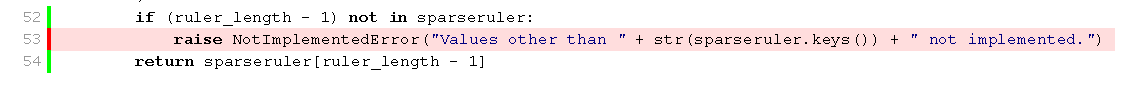
\includegraphics[width=\textwidth]{fig_branch_coverage.pdf}
    \caption{Coverage output of a branch that is never taken}
    \label{fig:coverage_branch}
\end{figure}

\subsection{Integration tests}
Integration tests verify the working of the complete system, or a few modules working together.


\end{document}
